\documentclass[a4paper]{article}

% Packages
\usepackage{geometry}
\geometry{left=1.5cm, right=1.5cm, top=2.54cm, bottom=2.54cm}
\usepackage{graphicx, hyperref, setspace, amsmath, amssymb, titlesec, fancyhdr, multicol, parskip, indentfirst, etoolbox, caption, cite, hyperref, xcolor}

\usepackage{subcaption} % Add to preamble


\usepackage{hyperref}
\hypersetup{
    colorlinks=true,
    linkcolor=blue,
    filecolor=magenta,      
    urlcolor=cyan,
    pdftitle={Overleaf Example},
    pdfpagemode=FullScreen,
    }

\urlstyle{same}

% Title Formatting
\titleformat{\section}{\centering\large\scshape}{\thesection}{1em}{}
\titleformat{\subsection}{\normalsize\bfseries}{\thesubsection.}{1em}{}
\setstretch{1.0} % Keep single spacing
\setlength{\parskip}{6pt} % Space between paragraphs
\titlespacing{\section}{0pt}{6pt}{6pt}
\titlespacing{\subsection}{0pt}{6pt}{6pt}
\titlespacing{\subsubsection}{0pt}{6pt}{6pt}
% Document Title
\title{
    \textbf{ Amazon Sales Product and Customer Personality Analysis} 
}

\date{} % No date
\captionsetup{labelfont={small,sc}, textfont={small,sc}}
% Section Numbering
% Define numbering format
\renewcommand{\thesection}{\Roman{section}.}
\renewcommand{\thesubsection}{\textit{\Alph{subsection}.}}
\renewcommand{\thesubsubsection}{\textit{\arabic{subsubsection}.}}
\renewcommand{\thetable}{\Roman{table}} % Set table numbering to Roman
\renewcommand{\thefigure}{\Roman{figure}} % Number figures in Roman numerals

% Make titles italic as well

\titleformat{\subsection}{\normalfont\large\itshape}{\thesubsection}{1em}{}
\titleformat{\subsubsection}{\normalfont\itshape}{\thesubsubsection}{1em}{}


\setcounter{page}{5}

% Fancy Header Configuration
\pagestyle{fancy}
\fancyhf{} % Clear all header/footer fields


% Default Header for Other Pages
\fancyhead[C]{\textbf{Data Science}}

\begin{document}

\maketitle
\vspace{-1.5cm}

% Authors Block
\begin{center}
    \textbf{Mahla Entezari}\\
    \textit{Shahid Beheshti University}\\
    \textit{Tehran, Iran}\\
    \textit{MahlaEntezari.sbu@gmail.com}
    \vfill
\end{center}


% Abstract (single-column)
\begin{abstract}
    In the realm of data science, every dataset is a gateway to a unique narrative. In this assignment, I embarked on an exploratory journey through Amazon's sales data—a dataset brimming with insights into customer behavior, product performance, and seasonal trends. This report is an account of the entire process, detailing how raw data was transformed into actionable knowledge through meticulous cleaning, analysis, and visualization.
    This report presents an in-depth analysis of sales data from Amazon to uncover insights about customer behavior, revenue trends, and product performance. The goal is to help stakeholders make data-driven decisions to improve marketing strategies, inventory planning, and revenue generation.
\end{abstract}


\singlespacing
\setlength{\parskip}{6pt}
\setlength{\parindent}{0.5cm}

 
\begin{multicols}{2}
\setlength{\columnsep}{0.5cm}


\section{Introduction}
Amazon, as a global e-commerce leader, generates enormous volumes of sales data daily. This project uses a publicly available dataset to investigate various dimensions of sales performance—from revenue trends to product category contributions and regional differences. Our approach builds on exploratory data analysis (EDA) techniques and statistical methods to draw meaningful conclusions.

The primary goal of this project is to:
\begin{itemize}
    \item Identify key trends and seasonal patterns in Amazon sales.
    \item Determine the top-performing product categories and regions.
    \item Uncover insights that can drive better marketing and inventory management decisions.
\end{itemize}


\section{Dataset}
\subsection{Amazon Sales Product}
\href{https://www.kaggle.com/datasets/mahlaentezari/amazon-dataset}{Amazon sales product dataset} contains product information, including ricing, discounts, ratings, reviews, and user interactions. The following are designed to analyze different aspects of the dataset using statistical methods.
Initial data exploration involved understanding the dataset's dimensions, checking for missing values, and ensuring data quality before moving into deeper analysis.

\subsection{Customer Personality Analysis}
\href{https://www.kaggle.com/datasets/imakash3011/customer-personality-analysis/data}{Customer Personality Analysis} is a detailed analysis of a company’s ideal customers. It helps a business to better understand its customers and makes it easier for them to modify products according to the specific needs, behaviors and concerns of different types of customers.

Customer personality analysis helps a business to modify its product based on its target customers from different types of customer segments. For example, instead of spending money to market a new product to every customer in the company’s database, a company can analyze which customer segment is most likely to buy the product and then market the product only on that particular segment.


\section{Methods}
Our methodology began with a thorough data preprocessing phase, followed by a comprehensive exploratory analysis. 

\subsection{Data Loading and Exploration}
The first step was to load the dataset and get acquainted with its structure. The dataset, acquired from a public source on Kaggle, contained detailed sales information. Using Python's \texttt{pandas} library, I quickly inspected the data to understand its dimensions and to identify any immediate issues such as missing values or duplicates.

\subsubsection{Initial Data Inspection}
I began by checking the overall shape and data types. This inspection revealed both numerical and categorical variables that required different preprocessing techniques. Missing values and anomalies were identified, setting the stage for a thorough data cleaning process.

\end{multicols} 

\begin{figure}[h]
    \centering
    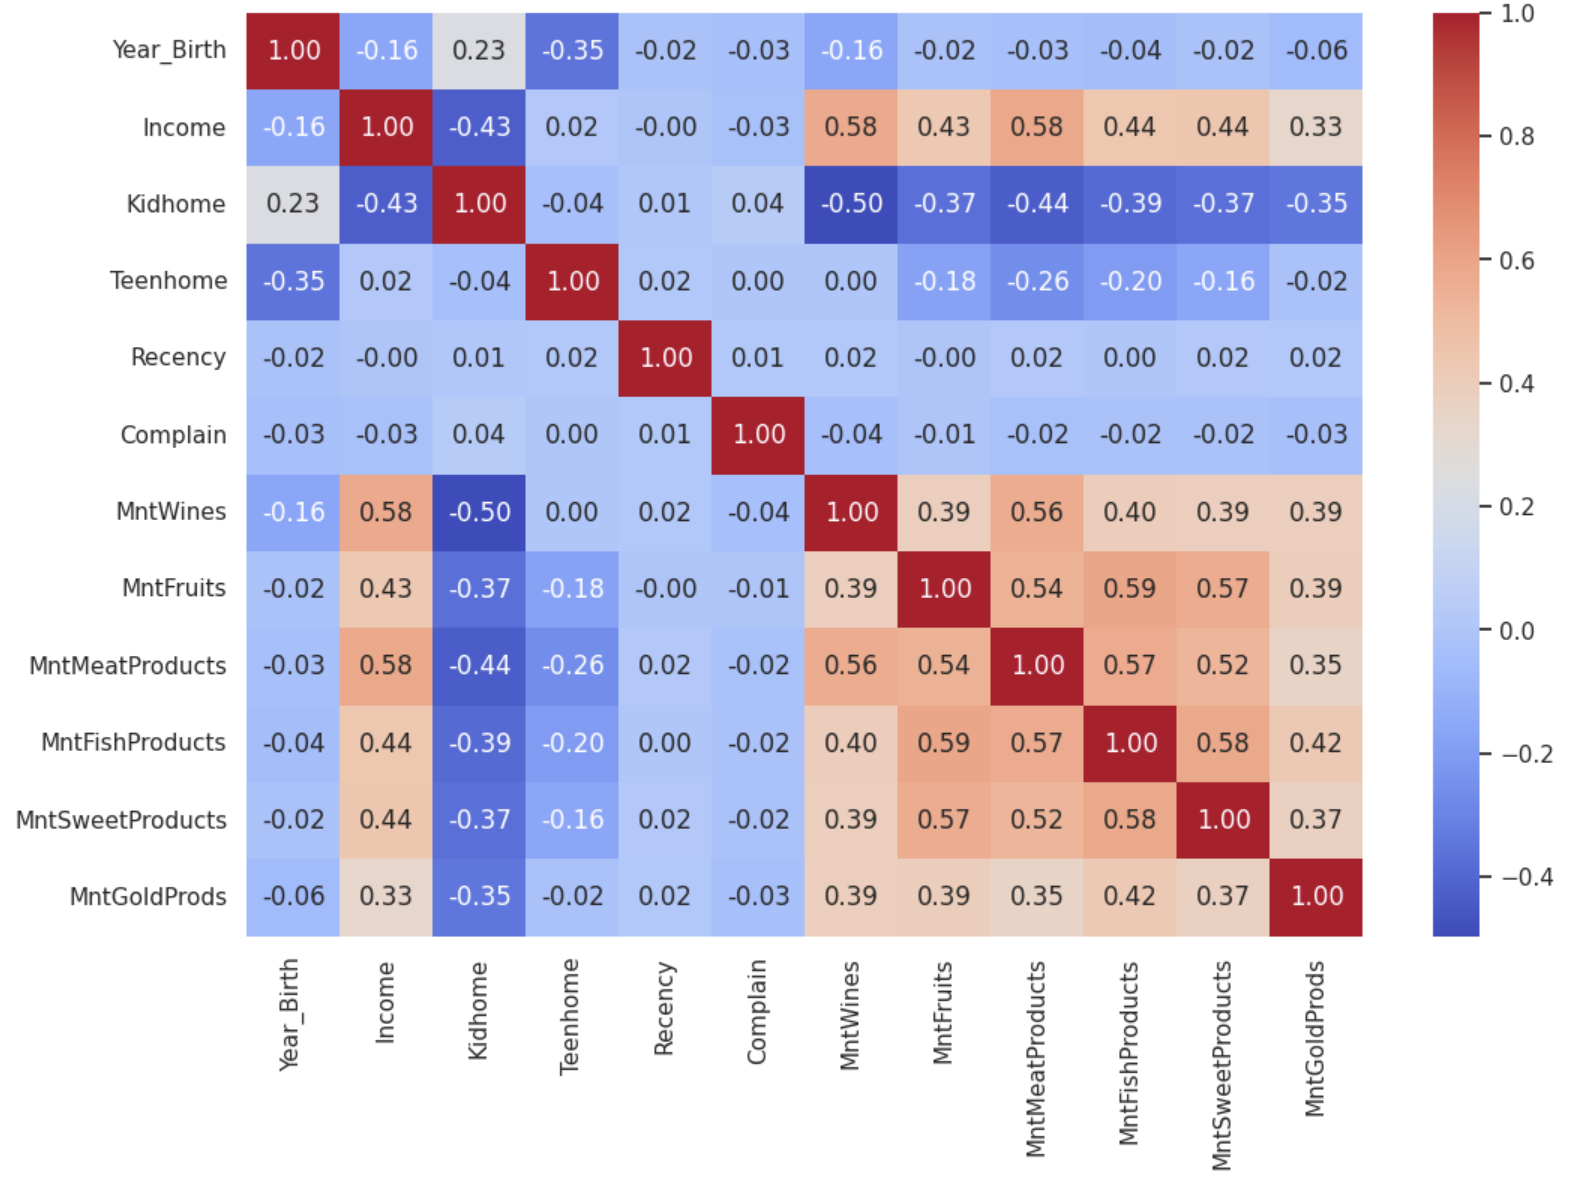
\includegraphics[width=0.7\textwidth]{Correlation Matrix.png}
    \caption{\textbf{Correlation Matrix}}
    
    Income is a significant factor influencing spending across various categories.
    
    Higher income correlates with higher spending, especially on wine and meat products.
    
    Kidhome negatively impacts spending, likely because households with more
    
    children may have different spending priorities.
    
    Teenhome has a minimal impact on spending, with slight negative 
    correlations in some categories.
    
    Recency and Complain do not show strong relationships with other variables, suggesting 
    
    they are less influential in this context.
    
    \label{fig:sales}
\end{figure}


\begin{multicols}{2}

\subsubsection{Data Cleaning and Feature Engineering}
Real-world data is rarely perfect. I addressed inconsistencies and missing values by removing duplicates and standardizing formats.
New features were engineered to enhance analysis, such as aggregating sales by month to capture seasonal patterns and creating derived variables that enriched the dataset.

This foundational work was essential for accurate downstream analysis.


\subsection{Uncovering Hidden Patterns}
With a cleaned dataset in hand, I dove into exploratory data analysis (EDA). The aim was to reveal underlying trends and relationships that could inform strategic decisions.


\subsection{Hypothesis tests}
I have conducted hypothesis tests to uncover insights about customer behaviors and characteristics.

\begin{minipage}{\columnwidth}
\captionof{table}{Shapiro-Wilk Test} 
\label{table:table1}
\centering
\begin{tabular}{|c|c|c|}
    \hline
    \textbf{Test} & \textbf{Test Statistic} & \textbf{P Value} \\
    \hline
    Kolmogorov-Smirnov& 0.3335 & $1.7108*10^{-285}$ \\
    Shapiro-Wilk & 0.4166 & $2.1882*10^{-70}$ \\
    \hline
\end{tabular}
\end{minipage}


Kolmogorov-Smirnov Test: Reject the null hypothesis. The data is not normally distributed.

Shapiro-Wilk Test: Reject the null hypothesis. The data is not normally distributed.

The KS statistic measures the maximum difference between the empirical distribution of the data and the theoretical normal distribution.
The Shapiro-Wilk Test is more sensitive to deviations from normality, especially for small to moderate sample sizes.
A p-value less than the significance level (a=0.05) indicates that the data significantly deviates from a normal distribution.

Conclusion: Reject the null hypothesis. The data is not normally distributed.


\end{multicols}

\section{Visualization}
it’s essential to understand the dataset’s structure and the relationships between variables. Begin by exploring the data through appropriate visualizations. This process will help us identify patterns, detect outliers, and formulate meaningful hypotheses.
Utilize various plots to explore relationships between variables. For
guidance on selecting suitable visualizations, refer to \href{https://www.data-to-viz.com/}{From Data to Viz} , a resource that assists in choosing the appropriate chart types based on our data.
To effectively communicate these insights, I employed various visualizations. Scatter plots, bar charts, and heatmaps transformed complex numerical relationships into intuitive graphics, each telling a part of the story.

\begin{figure}[h]
    \centering
    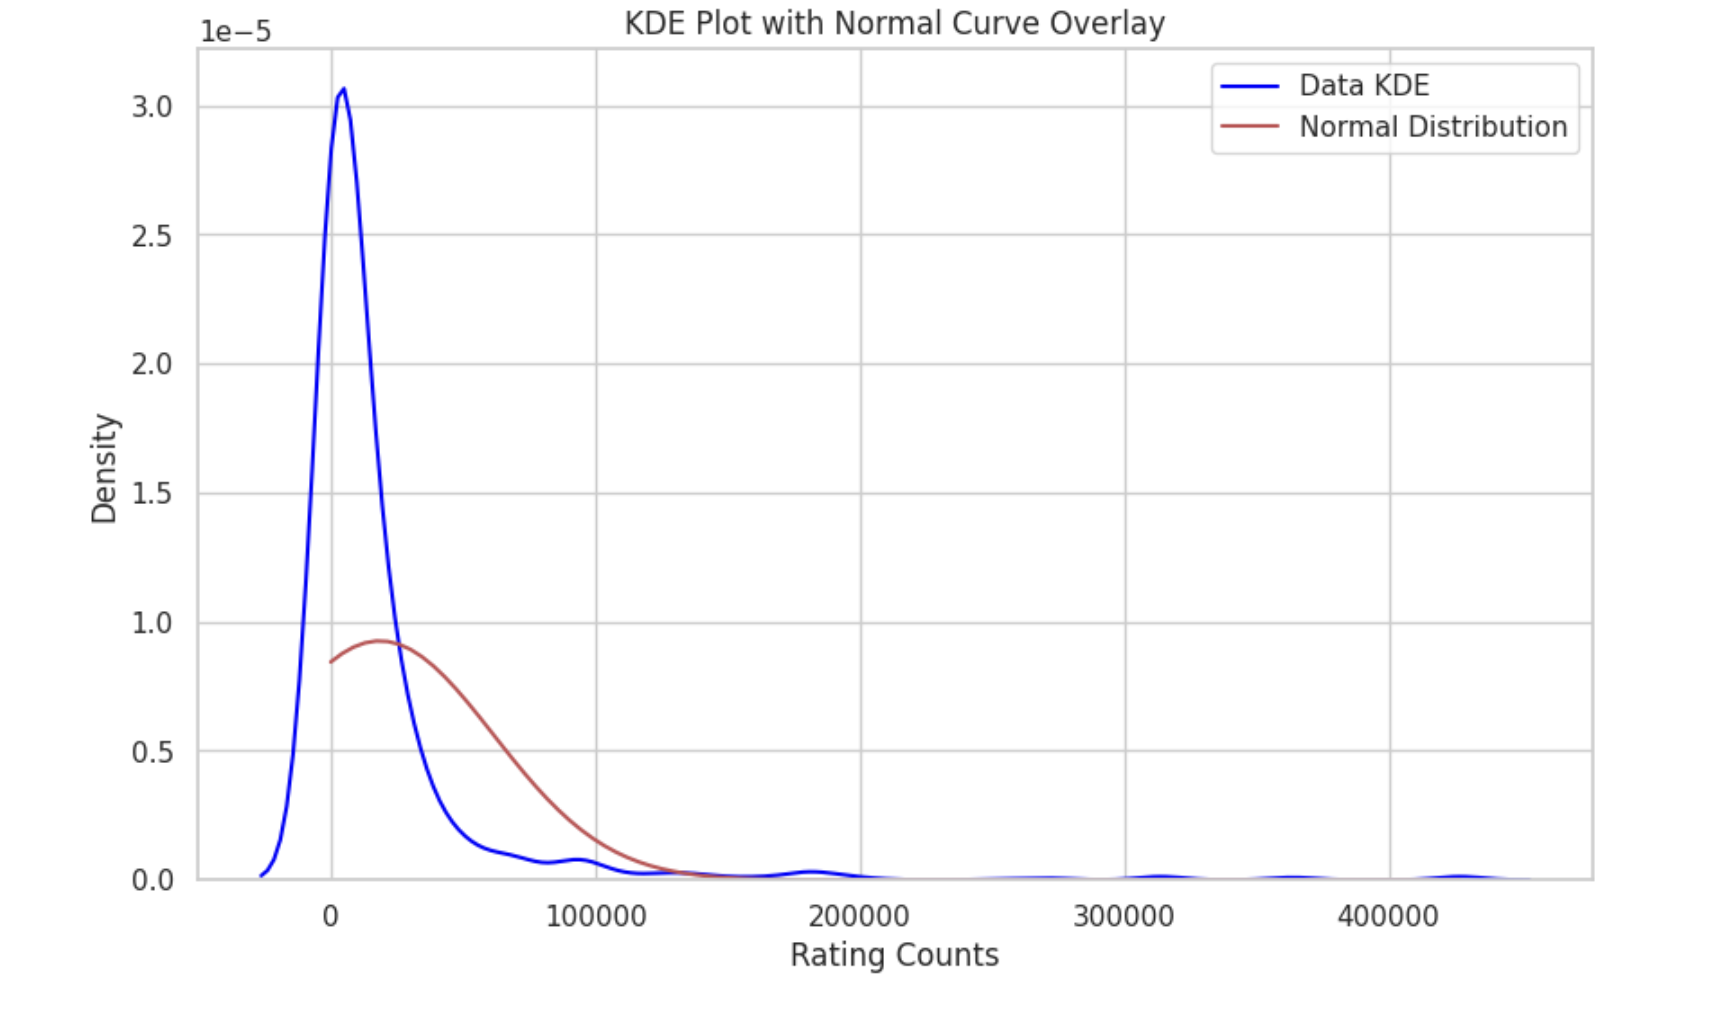
\includegraphics[width=0.5\textwidth]{KDE Plot with Normal Curve Overlay.png}
    \caption{\textbf{KDE plot of sales data with normal distribution curve}}
    Since the blue curve deviates significantly from the red curve:\
    The data is not normally distributed.
    The data likely has skewness, kurtosis, or outliers that cause it to deviate from a normal distribution.
    \label{fig:sales}
\end{figure}


\subsection{Histograms}
\begin{figure}[h]
    \centering
    \begin{subfigure}{0.3\textwidth}
        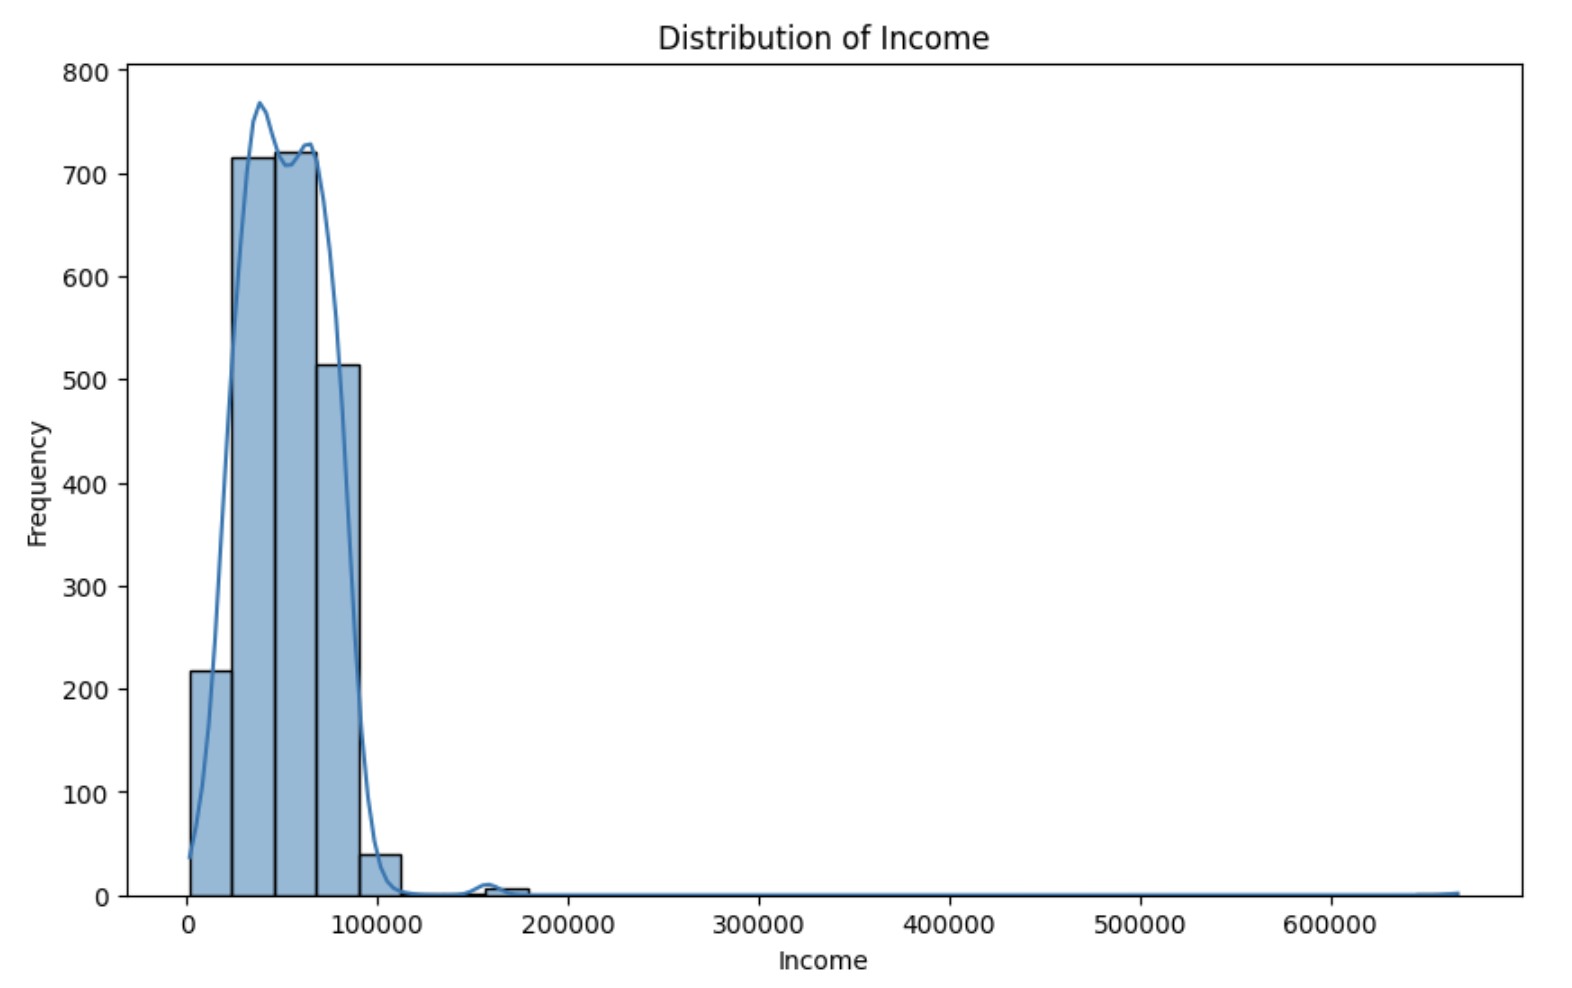
\includegraphics[width=\linewidth]{Distribution of Income.png}
        \caption{Distribution of Income}
        \label{fig:sub1}
    \end{subfigure}
    \hfill
    \begin{subfigure}{0.3\textwidth}
        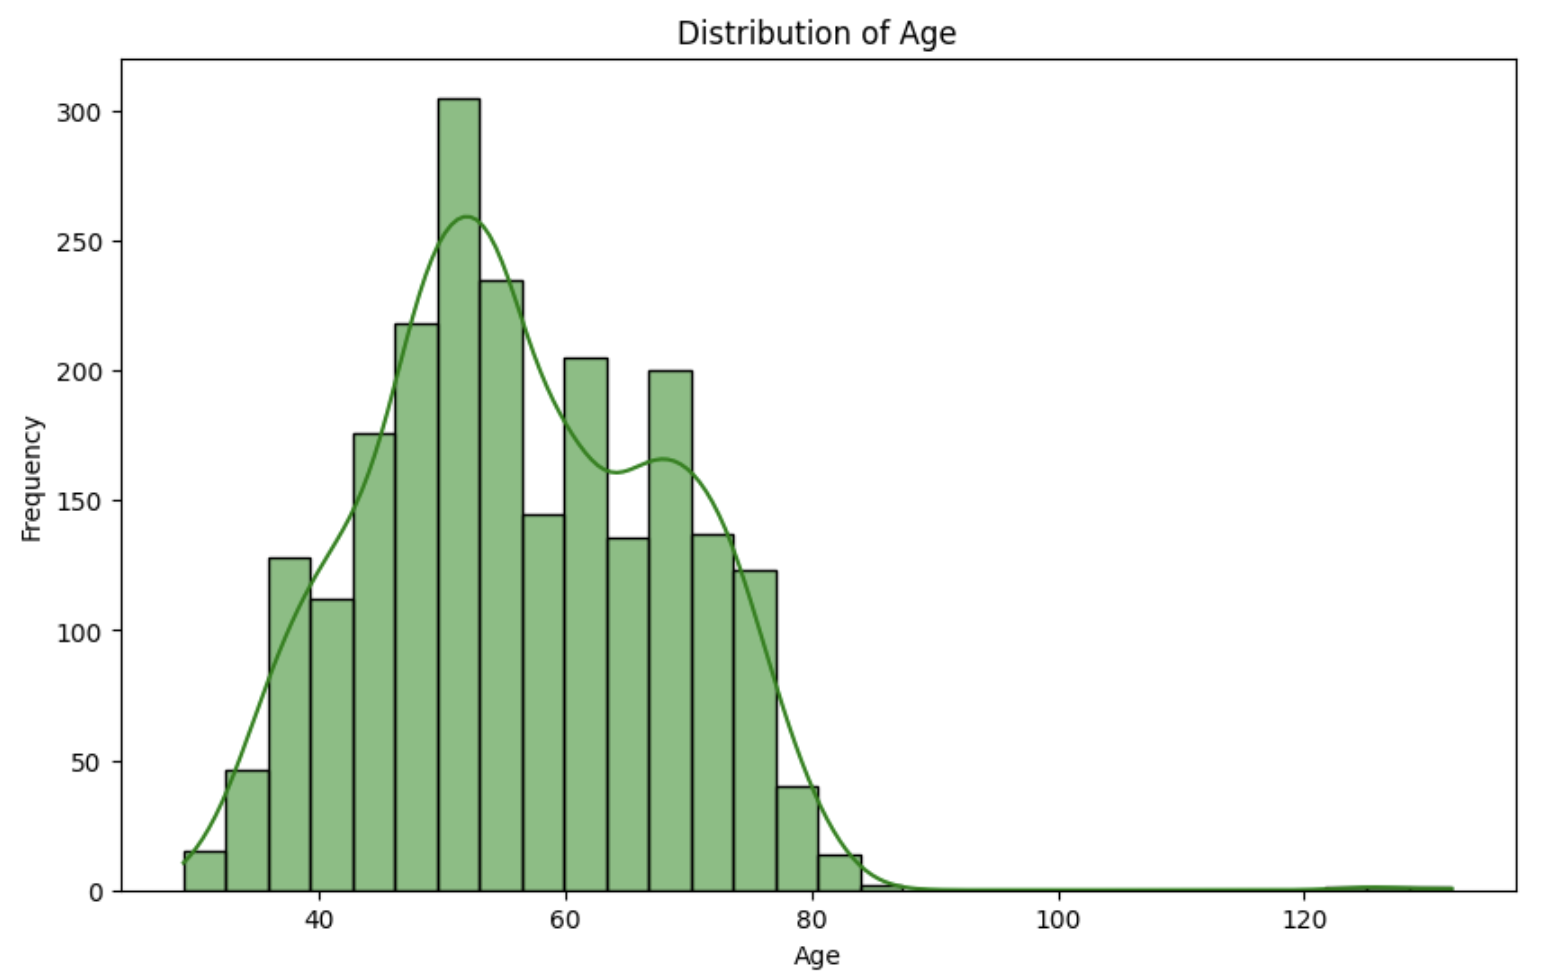
\includegraphics[width=\linewidth]{Distribution of Age.png}
        \caption{Distribution of Age}
        \label{fig:sub2}
    \end{subfigure}
    \hfill
    \begin{subfigure}{0.3\textwidth}
        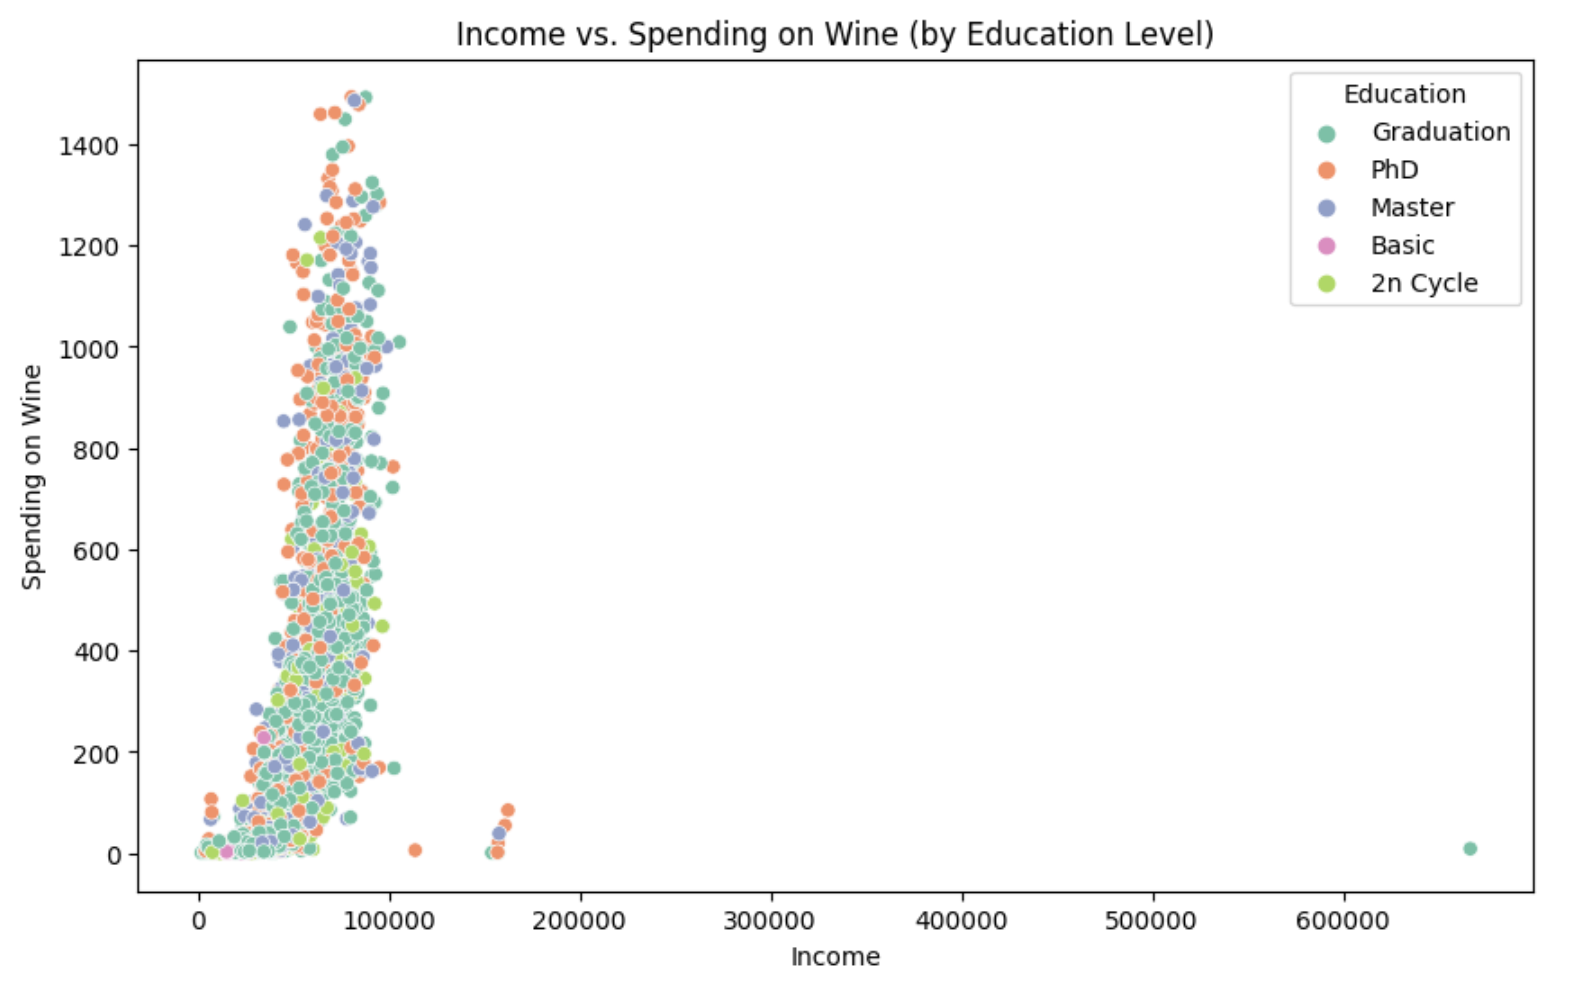
\includegraphics[width=\linewidth]{Income vs. Spending on Wine (by Education Level).png}
        \caption{Income vs. Spending on Wine}
        \label{fig:sub3}
    \end{subfigure}
    \caption{Some histograms for visualization}
    \label{fig:multi}
\end{figure}


\begin{multicols}{2} 

Distribution A is right-skewed, meaning most customers have incomes in the lower to mid-range (0 to 200,000).
There is a long tail on the right side, indicating a few customers with very high incomes (above 400,000).
The highest frequency of customers falls in the lower income ranges (0 to 100,000).
This suggests that the majority of customers have moderate incomes.
There are a few customers with very high incomes (above 400,000), which are represented by the long tail on the right.


The distribution B is approximately normal, with most customers aged between 40 and 60 years.
The frequency of customers decreases as age increases beyond 60 years.
The highest frequency of customers falls in the middle age ranges (40 to 60 years).
This suggests that the majority of customers are middle-aged.
There are a few customers who are very young (below 40 years) or very old (above 80 years), but these are relatively rare.


In the plot C, there is a positive correlation between income and spending on wine: as income increases, spending on wine tends to increase.
Higher-income customers (above 200,000) generally spend more on wine compared to lower-income customers.
Customers with higher education levels (PhD, Master) tend to have higher incomes and spend more on wine.
Customers with basic education tend to have lower incomes and spend less on wine.
There are a few customers with very high incomes (above 400,000) who spend significantly more on wine than the average customer.


\end{multicols}

\subsection{Bar Plots}
\begin{figure}[h]
    \centering
    \begin{subfigure}{0.32\textwidth}
        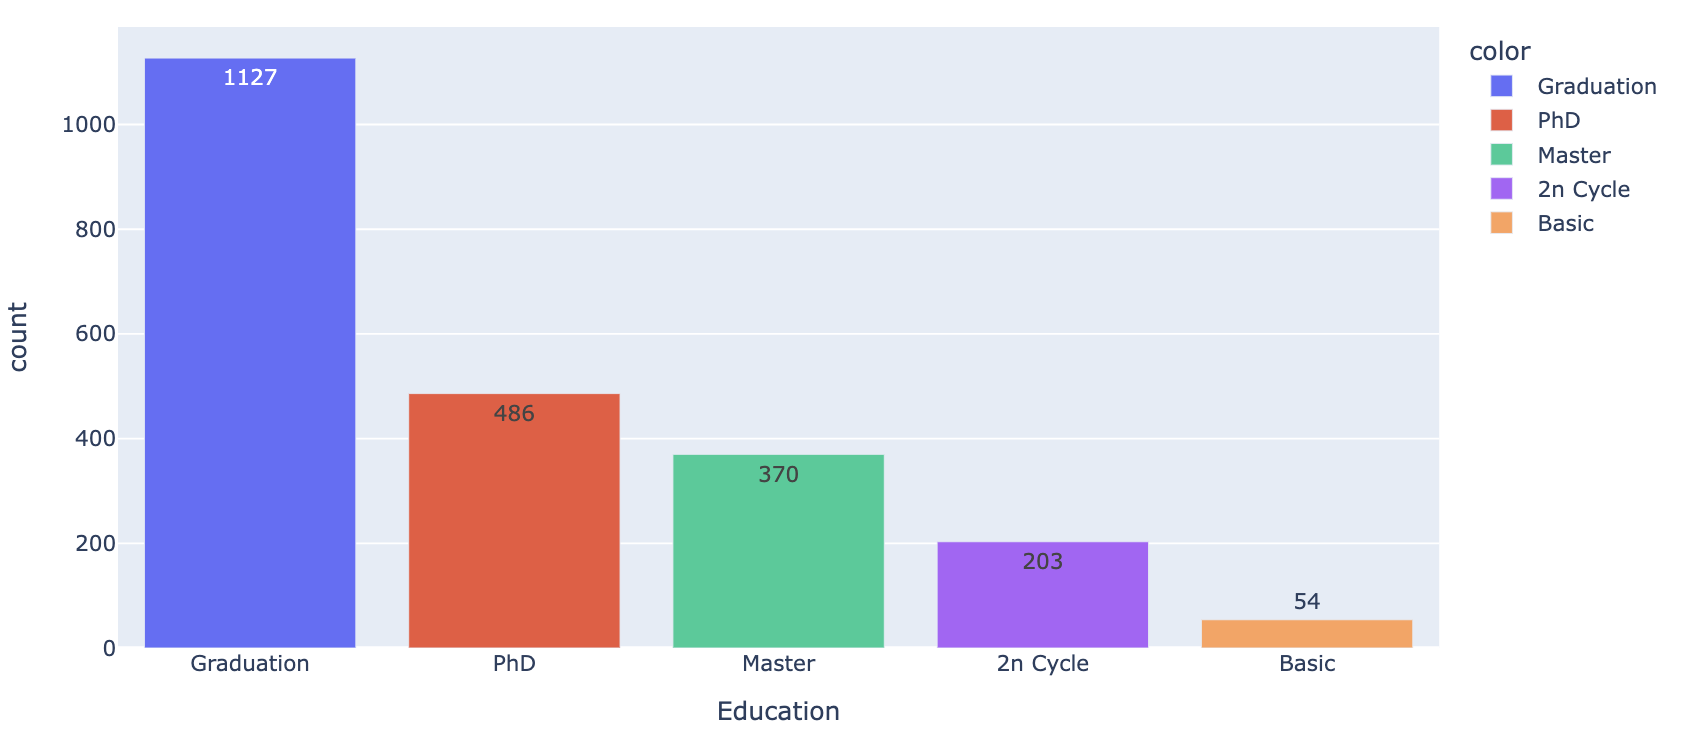
\includegraphics[width=\linewidth]{Distribution of Customer Education Level.png}
        \caption{Distribution of Customer Education Level}
        \label{fig:sub1}
    \end{subfigure}
    \hfill
    \begin{subfigure}{0.32\textwidth}
        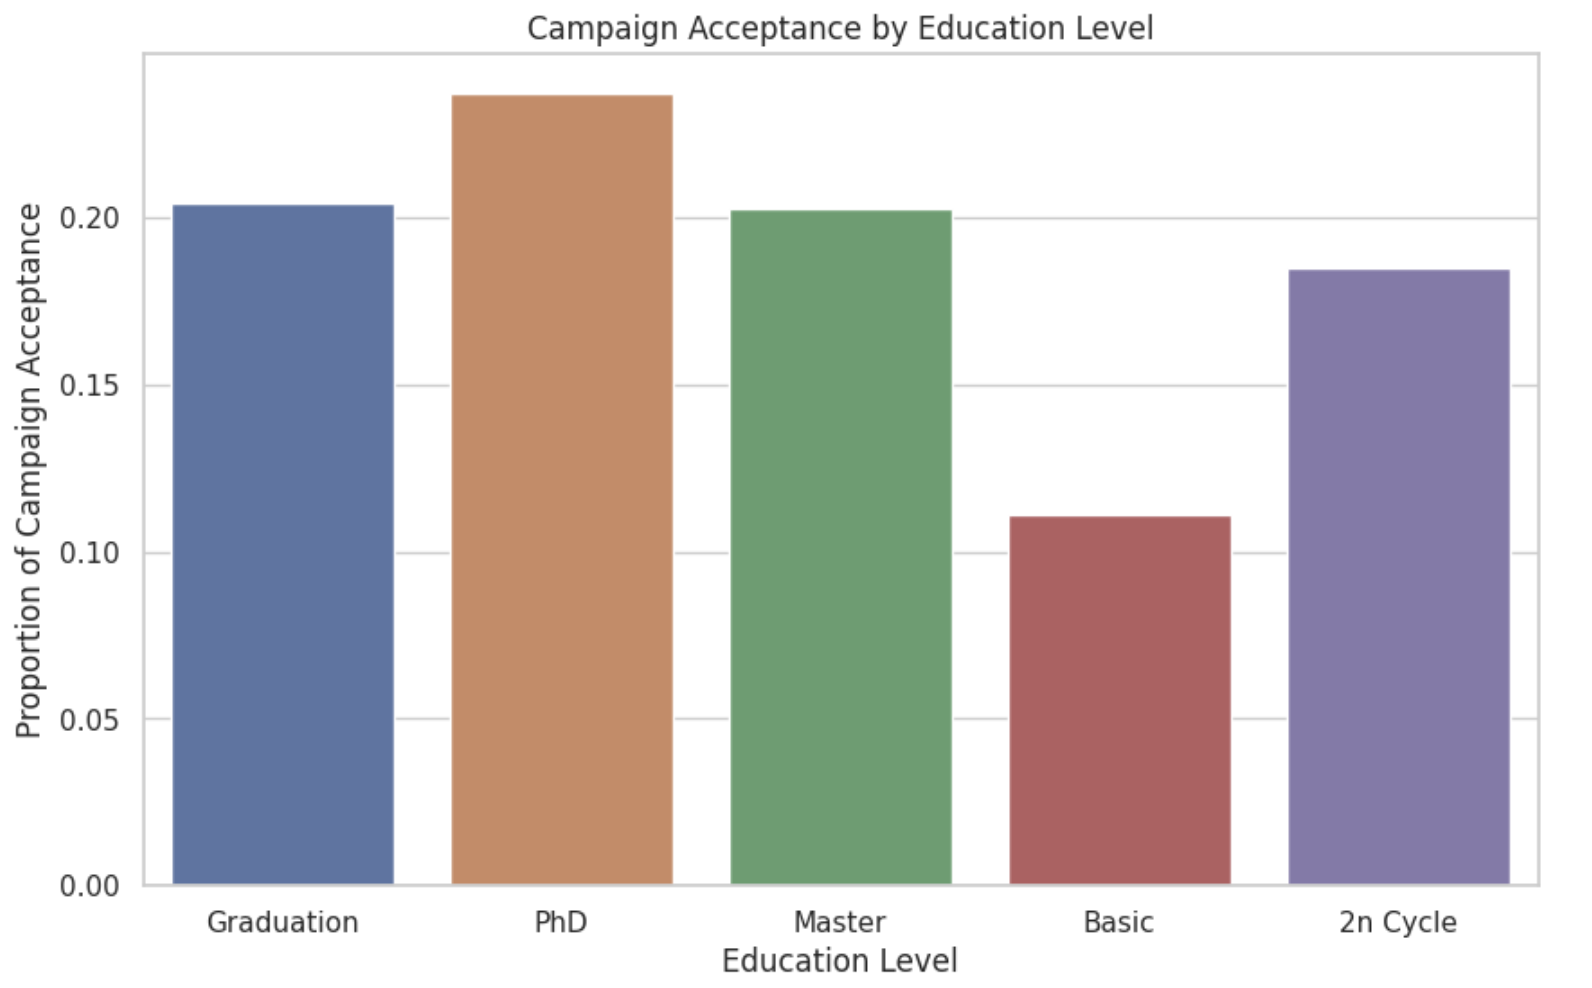
\includegraphics[width=\linewidth]{Campaign Acceptance by Education Level.png}
        \caption{Campaign Acceptance by Education Level}
        \label{fig:sub2}
    \end{subfigure}
    \hfill
    \begin{subfigure}{0.32\textwidth}
        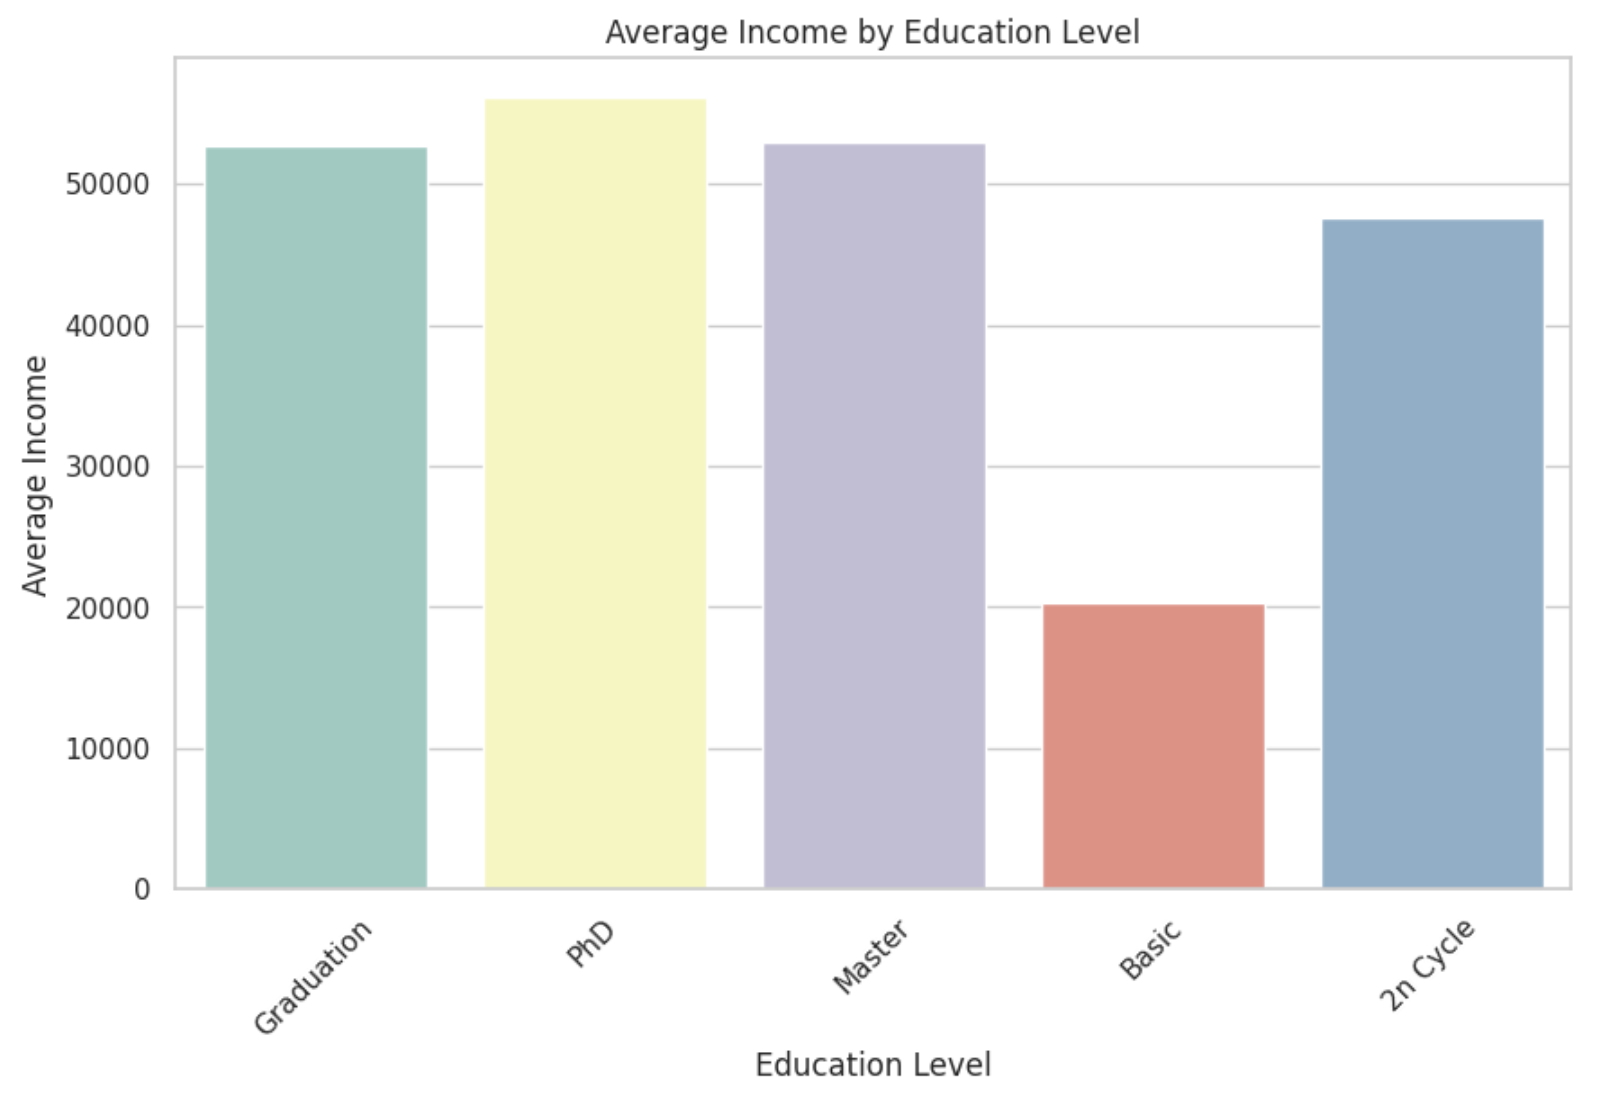
\includegraphics[width=\linewidth]{Average Income by Education Level.png}
        \caption{Average Income by Education Level}
        \label{fig:sub3}
    \end{subfigure}
    \caption{Some bar plots for visualization}
    \label{fig:multi}
\end{figure}



\begin{multicols}{2} 

In plot A, the Graduation category has the highest count (1127 customers), indicating that most customers have a Graduation-level education.\
This is followed by PhD (486 customers) and Master (370 customers).\
The 2n Cycle and Basic categories have significantly fewer customers (203 and 54, respectively).\
These education levels represent a smaller proportion of the customer base.\
The distribution is right-skewed, with most customers having higher education levels (Graduation, PhD, Master).


In plot B, customers with higher education levels (Graduation, PhD) are more likely to accept promotional campaigns compared to those with lower education levels (Basic, 2n Cycle).\
The Basic education group has the lowest campaign acceptance rate, suggesting that customers with basic education are less likely to respond to promotional campaigns.


In plot C, higher Education, Higher Income: There is a clear trend where higher levels of education correspond to higher average incomes. This is consistent with general economic theories that more education often leads to better-paying jobs.\
PhD and Master Degrees: These advanced degrees are associated with the highest incomes, likely due to the specialized skills and knowledge they provide, which are in demand in the job market.\

Basic and 2n Cycle: These education levels are associated with lower incomes, possibly because they may lead to jobs that require less specialized skills and are more entry-level.\
Encourage individuals to pursue higher education, particularly advanced degrees like Master's and PhDs, to increase their earning potential.\
Provide financial support for students aiming for higher education to make it more accessible.\
Offer guidance to students and professionals on the potential income benefits of advanced degrees and specialized training.



\end{multicols}


\begin{figure}[h]
    \centering
    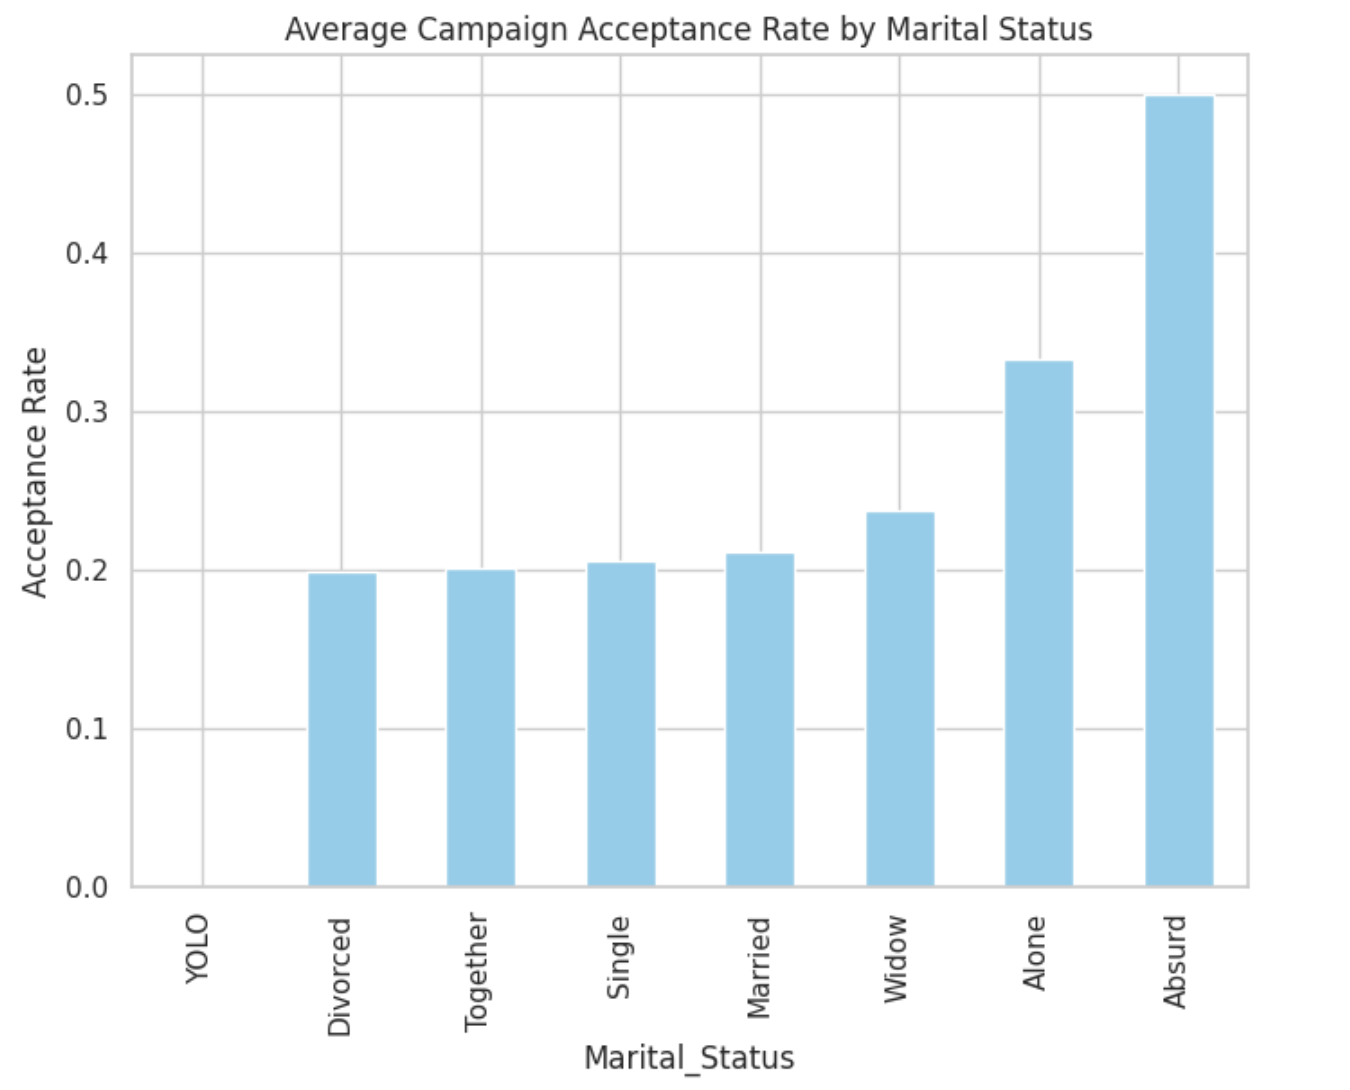
\includegraphics[width=0.55\textwidth]{Average Campaign Acceptance Rate by Marital Status.png}
    \caption{\textbf{Average Campaign Acceptance Rate by Marital Status}}

    \label{fig:sales}
\end{figure}


\subsection{Box Plots}
\begin{figure}[h]
    \centering
    \begin{subfigure}{0.3\textwidth}
        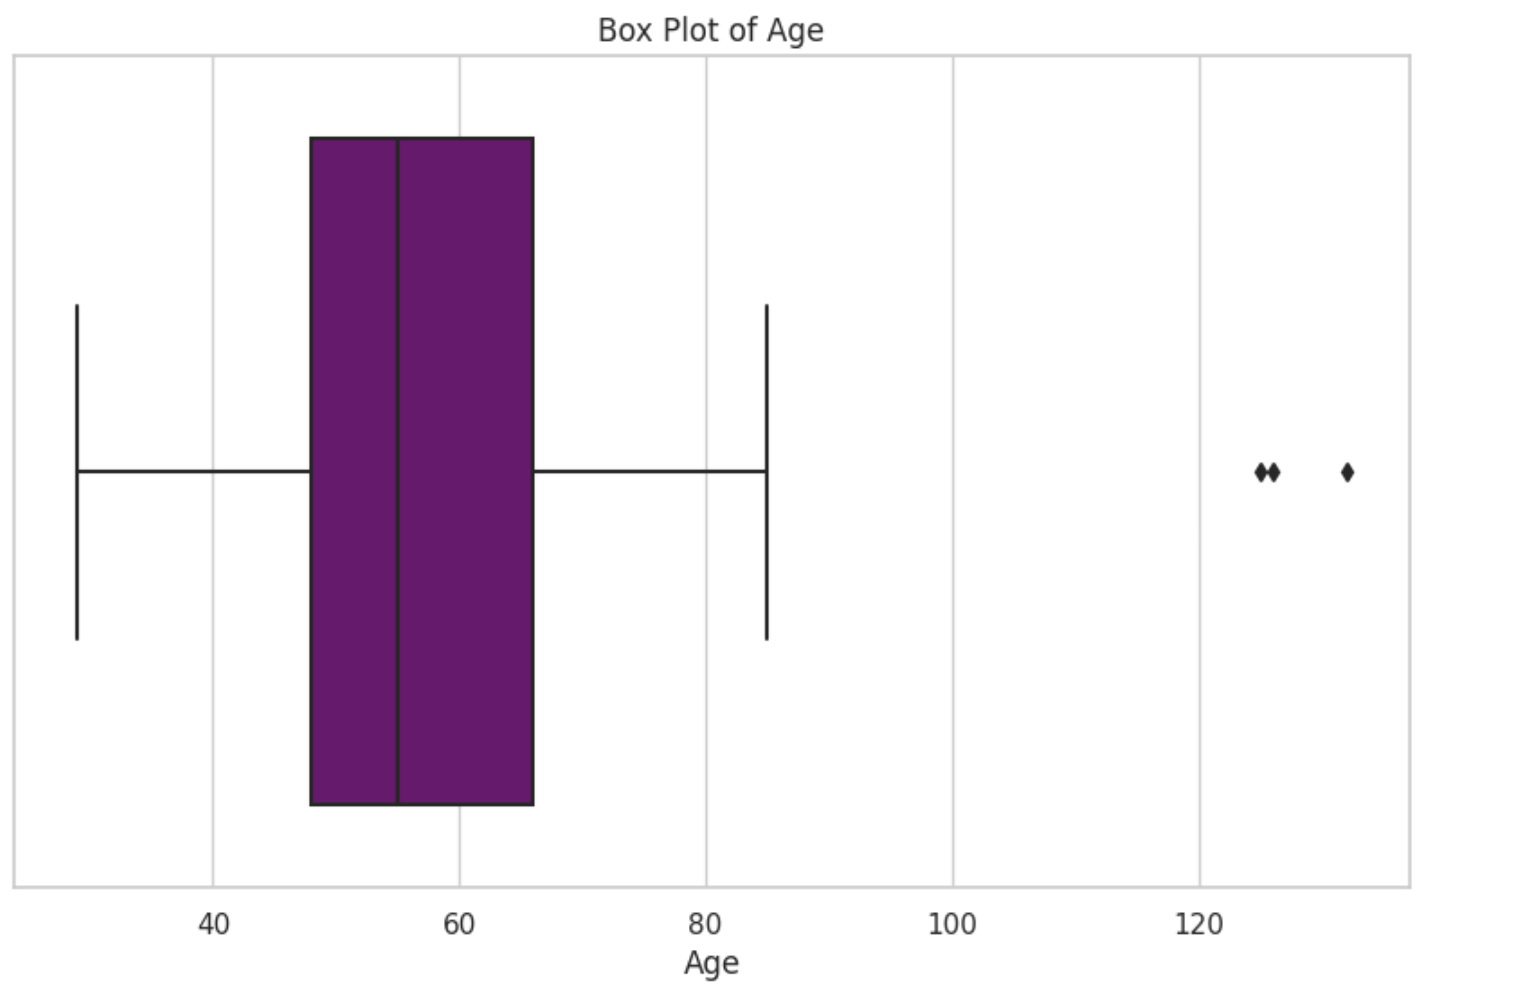
\includegraphics[width=\linewidth]{Box Plot of Age.png}
        \caption{Box Plot of Age}
        \label{fig:sub1}
    \end{subfigure}
    \hfill
    \begin{subfigure}{0.3\textwidth}
        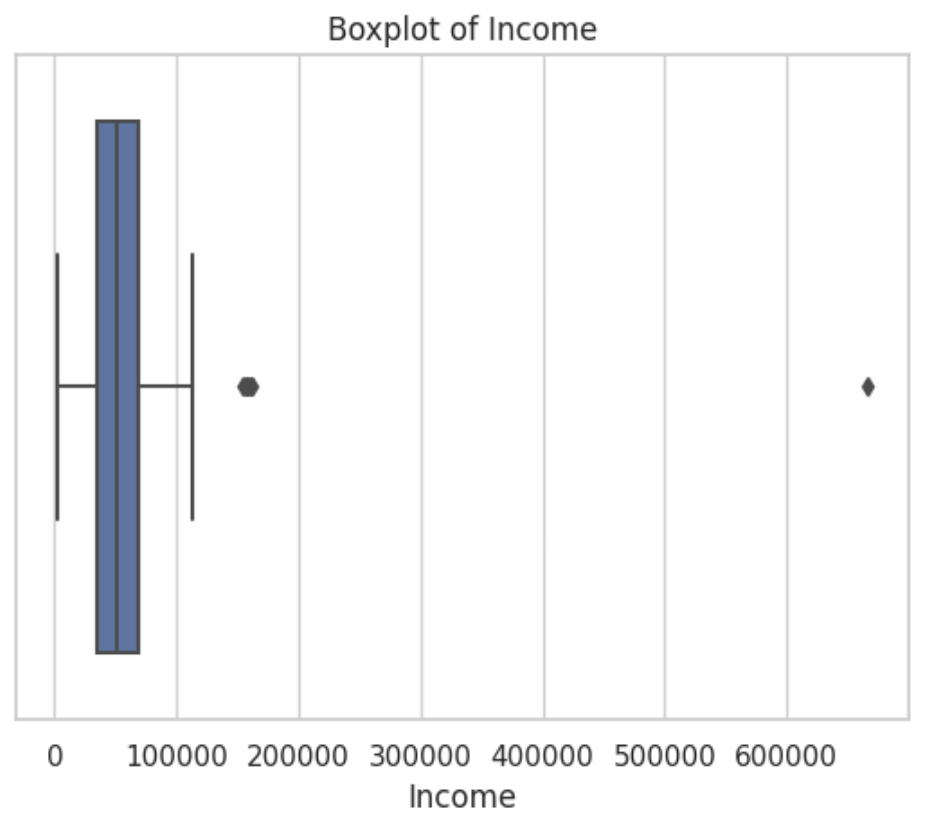
\includegraphics[width=\linewidth]{Boxplot of Income.png}
        \caption{Boxplot of Income}
        \label{fig:sub2}
    \end{subfigure}
    \hfill
    \begin{subfigure}{0.3\textwidth}
        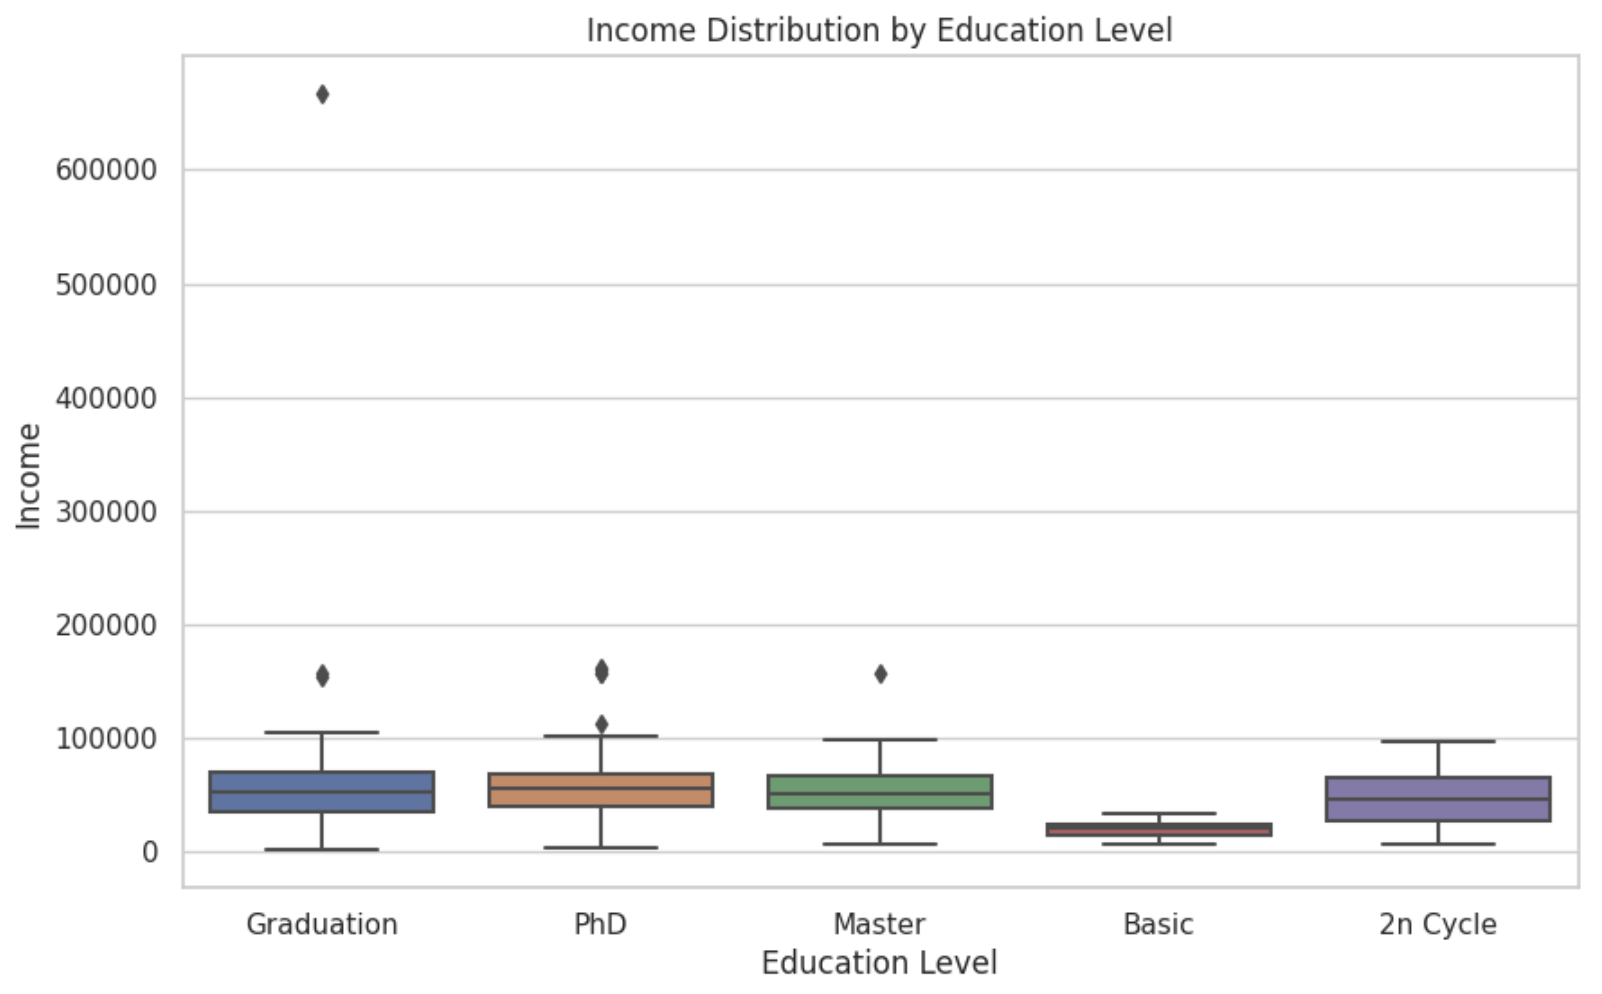
\includegraphics[width=\linewidth]{Income Distribution by Education Level.png}
        \caption{Income Distribution by Education Level}
        \label{fig:sub3}
    \end{subfigure}
    \hfill
    \begin{subfigure}{0.3\textwidth}
        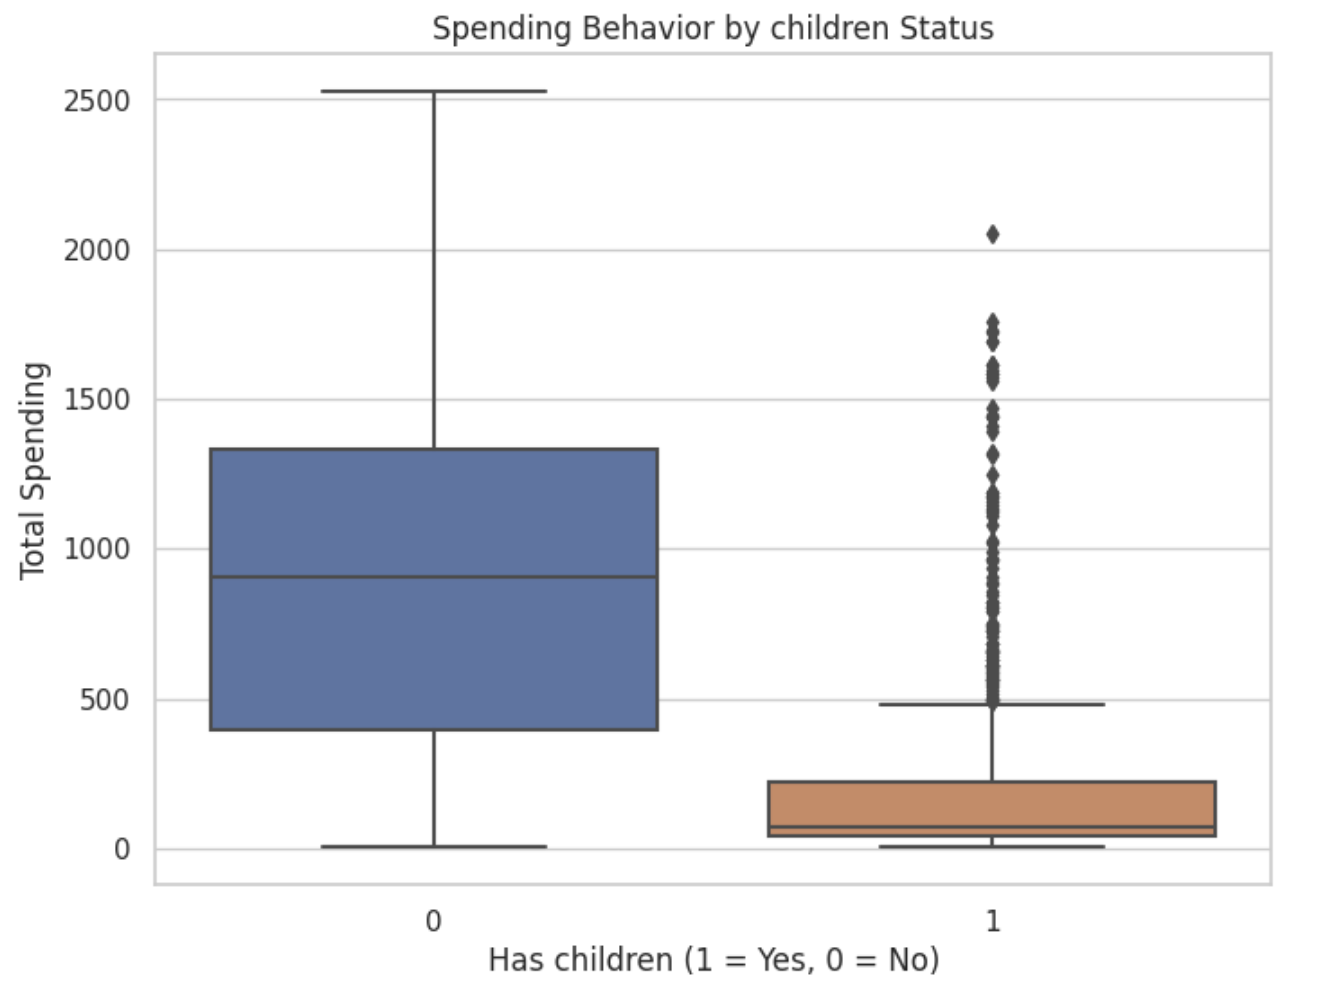
\includegraphics[width=\linewidth]{Spending Behavior by children Status.png}
        \caption{Spending Behavior by children Status}
        \label{fig:sub4}
    \end{subfigure}
    \hfill
    \begin{subfigure}{0.3\textwidth}
        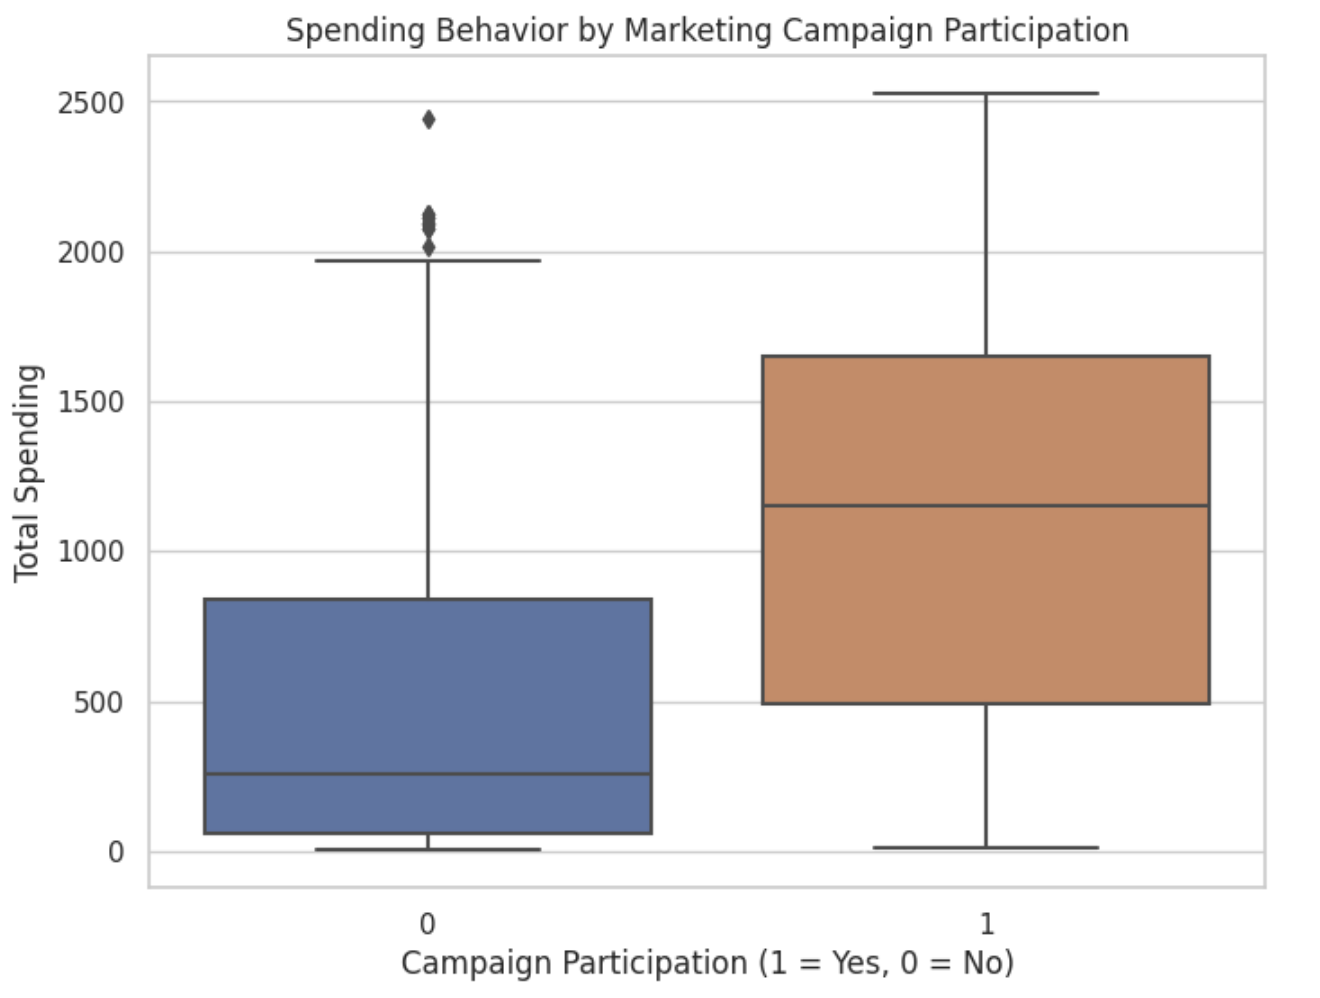
\includegraphics[width=\linewidth]{Spending Behavior by Marketing Campaign Participation.png}
        \caption{Spending Behavior by Marketing Campaign Participation}
        \label{fig:sub5}
    \end{subfigure}
    \hfill
    \begin{subfigure}{0.3\textwidth}
        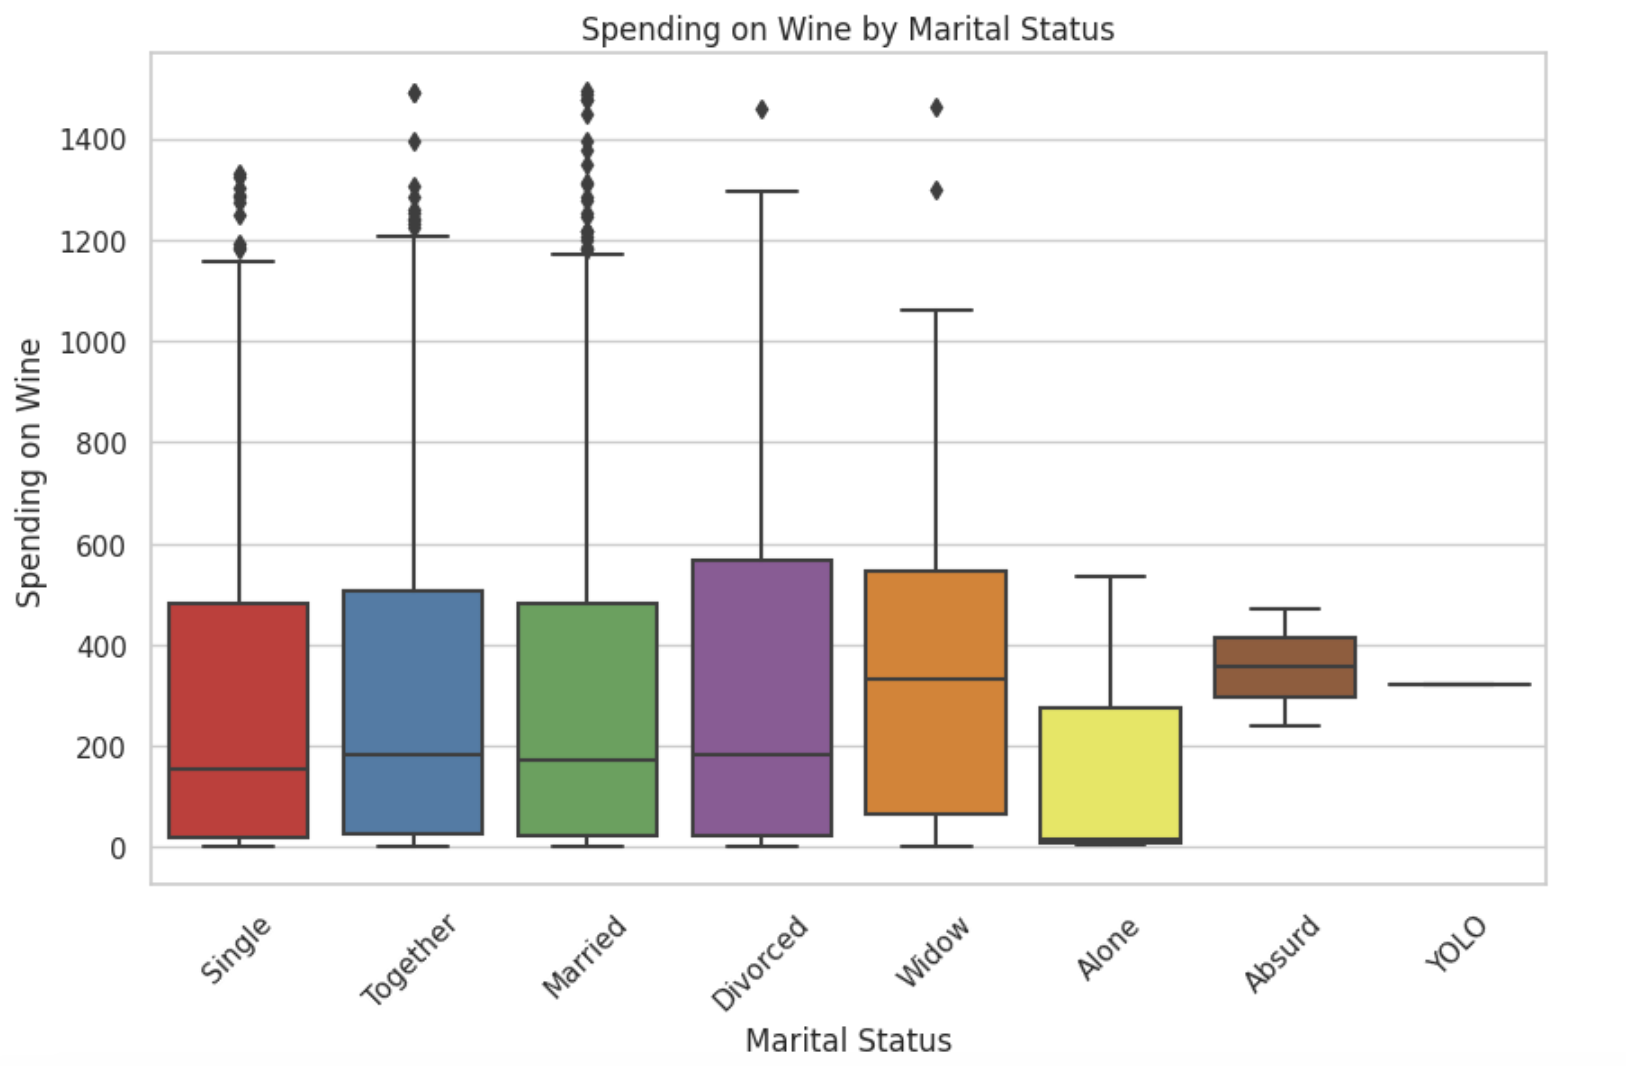
\includegraphics[width=\linewidth]{Spending on Wine by Marital Status.png}
        \caption{Spending on Wine by Marital Status}
        \label{fig:sub6}
    \end{subfigure}
    \caption{Some box plots for visualization}
    \label{fig:multi}
\end{figure}

\begin{multicols}{2} 

The box plot A provides a visual summary of the age distribution, showing the central tendency, spread, and presence of outliers.
The length of the box and whiskers indicates the variability in age. A longer box or whiskers suggest greater variability.
Outliers can indicate individuals with exceptionally high or low ages compared to the general population.


In box plot B, the median income (the line inside the box) is around 50,000 to 100,000, indicating that half of the customers earn less than this amount, and half earn more.
The IQR (the box) spans from approximately 25,000 to 150,000, representing the middle 50\% of customer incomes.
There are several high-income outliers (above 400,000), indicating that a small proportion of customers earn significantly more than the majority.
The distribution is right-skewed, as the right whisker is longer than the left, and there are high-income outliers.


In box plot C, higher education (PhD/Master) correlates with higher incomes, aligning with global trends.
High-income groups (PhD/Master) may respond better to premium products.
Lower-income groups (Basic/2n Cycle) may prioritize affordability.
Encouraging education could improve earning potential, especially for the Basic and 2n Cycle groups.
This plot confirms that education level is a strong predictor of income, which can guide business strategies (pricing, promotions) and social policies. For instance, a wine company might target PhD/Master customers with high-end offerings, while budget-friendly options could appeal to the Basic group.


In plot D, customers without children have higher median spending compared to customers with children.
The wider IQR for customers without children suggests greater variability in their spending behavior.
The presence of outliers indicates that some customers in both groups spend significantly more than the typical customer.


In plot E, target PhD/Master customers with premium products (they have higher disposable income).
For Basic/2n Cycle groups, emphasize affordability or payment plans.
The plot validates that advanced education correlates with higher earnings.
The wide income ranges in higher education suggest that factors beyond education (industry, experience) also play a role.
Confirms that education level is a strong predictor of income, useful for segmentation.
While education matters, other factors (job sector, geography) likely contribute to income variability within groups.

From the plot F, following results can be concluded:\

Married and Together: These groups likely have higher disposable income or more social occasions involving wine, leading to higher spending.\

Single and Divorced: These groups might have moderate social activities or different spending priorities, resulting in moderate wine spending.\

Widow and Alone: These groups might have lower spending due to less social engagement or different lifestyle choices.\

Absurd and VOLO: These categories might need further investigation to understand their relevance and why they show minimal spending.




\section{Results}

Most customers in the dataset have incomes in the lower to mid-range (0 to 200,000).
Marketing strategies should focus on this majority group, as they represent the largest customer base.
A small proportion of customers have very high incomes (above 400,000).
These high-income customers represent a premium segment that may require specialized marketing strategies (luxury products or exclusive offers).
For moderate-income customers, focus on affordability and value-for-money products.
For high-income customers, focus on premium products, personalized services, and exclusive offers.


Most customers in the dataset are middle-aged (40 to 60 years).
Marketing campaigns should focus on this demographic, as they represent the largest customer base.
A small proportion of customers are very young (below 40 years) or very old (above 80 years).
These customers represent niche segments that may require specialized marketing strategies.
For middle-aged customers, focus on products and services that cater to their lifestyle and preferences (family-oriented products, health and wellness).
For very young or very old customers, consider niche products or services that meet their specific needs.


Customers with higher incomes are the primary spenders on wine.
Marketing campaigns for wine products should target higher-income customers.
Customers with advanced education levels (PhD, Master) tend to have higher incomes and spend more on wine.
Marketing campaigns should also consider targeting highly educated customers.
A small group of customers with very high incomes spends significantly more on wine.
These customers represent a premium segment that may require specialized marketing strategies (luxury wine offerings or exclusive deals).


Most customers in the dataset have Graduation, PhD, or Master-level education.
Marketing campaigns should focus on these groups, as they represent the largest customer base.
Customers with 2n Cycle or Basic education levels are a smaller segment of the customer base.
These groups may require specialized marketing strategies tailored to their preferences and needs.
For highly educated customers (Graduation, PhD, Master), focus on premium products, advanced features, and value-added services.
For less educated customers (2n Cycle, Basic), focus on affordability, simplicity, and ease of use.



The majority of customers have incomes in the lower to mid-range (25,000 to 150,000).
Marketing strategies should focus on this majority group, as they represent the largest customer base.
A small proportion of customers have very high incomes (above 400,000).
These high-income customers represent a premium segment that may require specialized marketing strategies (luxury products or exclusive offers).
For moderate-income customers, focus on affordability and value-for-money products.
For high-income customers, focus on premium products, personalized services, and exclusive offers.



Encourage individuals to pursue higher education, particularly advanced degrees like Master's and PhDs, to increase their earning potential.
Provide financial support for students aiming for higher education to make it more accessible.
Offer guidance to students and professionals on the potential income benefits of advanced degrees and specialized training.



Focus marketing efforts on married and together individuals, as they show the highest spending on wine.
Consider promotions or discounts for single and divorced individuals to increase their spending on wine.
Investigate the reasons behind lower spending by widows and those who are alone to identify potential opportunities or barriers.
Check the data for categories like "Absurd" and "VOLO" to ensure they are correctly classified and understand their context.


Investigate the outliers to understand the reasons behind exceptionally high or low incomes and ages.
Use the income and age distribution to segment customers for targeted marketing strategies.


Focus campaigns on Married/Together customers for better conversion
Adjust messaging for singles\
Singles respond less - try different messaging or offer types\
Singles need different engagement strategies to boost response rates\
Consider merging small categories (like Alone with Single)
Remove the repetitive decimal points cluttering the visualization\
Remove or fix the Absurd/YOLO entries
Married couples are most responsive segment - prioritize them in campaigns\
Target Married/Together Customers most likely to respond - focus best offers here


The box plot and statistical test both confirm that customers with children spend differently than those without children.
Specifically, customers without children tend to spend more, while customers with children spend less on average.

Considering the results of this analytical project, can help in making informed decisions about pricing, product offerings, financial planning, services, and customer engagement strategies.


\begin{thebibliography}{9}

\bibitem{dataset}
Dataset available on Kaggle: ``Amazon Sales Analysis'' by MahlaEn. \textit{Available at:} \url{https://www.kaggle.com/datasets/mahlaentezari/amazon-dataset}.

\bibitem{dataset}
Dataset available on Kaggle: ``Customer Personality Analysis'' by imakash3011. \textit{Available at:} \url{https://www.kaggle.com/datasets/imakash3011/customer-personality-analysis/data}.

\bibitem{dataset}
Plots for data visualization. \textit{Available at:} \url{https://www.data-to-viz.com/}.


\bibitem{Statistics}
cole nussbaumer knaflic. \textit{Storytelling with data } a data visualization guide for business.

\end{thebibliography}

\end{multicols}
\end{document}